%!TEX TS-program = xelatex
 
% Этот шаблон документа разработан в 2014 году
% Данилом Фёдоровых (danil@fedorovykh.ru) 
% для использования в курсе 
% <<Документы и презентации в \LaTeX>>, записанном НИУ ВШЭ
% для Coursera.org: http://coursera.org/course/latex .
% Исходная версия шаблона --- 
% https://www.writelatex.com/coursera/latex/5.2.2
 
\documentclass[a4paper,12pt]{article}
 
%%% Работа с русским языком
\usepackage[english,russian]{babel}   %% загружает пакет многоязыковой вёрстки
\usepackage{fontspec}      %% подготавливает загрузку шрифтов Open Type, True Type и др.
\defaultfontfeatures{Ligatures={TeX},Renderer=Basic}  %% свойства шрифтов по умолчанию
\setmainfont[Ligatures={TeX,Historic}]{Times New Roman} %% задаёт основной шрифт документа
\setsansfont{Comic Sans MS}                    %% задаёт шрифт без засечек
\setmonofont{Courier New}
\usepackage{indentfirst}
\frenchspacing
 
%%% Дополнительная работа с математикой
\usepackage{amsmath,amsfonts,amssymb,amsthm,mathtools} % AMS
\usepackage{icomma} % "Умная" запятая: $0,2$ --- число, $0, 2$ --- перечисление
 %% Номера формул
\mathtoolsset{showonlyrefs=true} % Показывать номера только у тех формул, на которые есть \eqref{} в тексте.

\author{Батарин Егор}
\title{Дифракция на ультразвуке}
\date{\today}
 
\begin{document} % конец преамбулы, начало документа
 
\maketitle
 


\section{Цель работы} 

Изучение дифракции света на синусоидальной акустической решетке и наблюдение фазовой решетки методом темного поля. 

\section{В работе используется}

Оптическая скамья, осветитель, два длиннофокусных объектива, кювета с жидкостью, кварцевый излучатель с микрометрическим винтом, генератор ультразвуковой частоты, линза, вертикальная нить на рейтере, микроскоп. 

\section{Теория}

В работе изучается дифракция света на фазовой решетке. Фазовая решетка создается в жидкости улттразвуковыми волнами и наблюдается методом темного поля. 



При прохождении УЗ волны через жидкость в ней возникают периодические оптические неоднородности, обусловленные разницей значений коэффициента преломления в областях сжатия и разряжения. Эти периодические неоднородности играют роль своеобразной дифракционной решетки.


Пусть УЗ волна распространяется вдоль оси $X$ в жидкости. В направлении $Z$ сквозь жидкость проходит световая волна, испытывающая дифракцию на акустической решетке. Поскольку скорость света значительно больше скорости звука, акустическую решетку можно считать неподвижной. Вызванное ультразвуком возмущение показателя преломления очень мало. Акустическую решетку можно рассматривать как \textbf{тонкий фазовый экран}. 

При небольших амплитудах звуковой волны показатель преломления жидкости n меняется по закону 

\begin{equation}
n = n_0 (1 + m \cos{\Omega x}),
\label{eq2}
\end{equation}

где $\Omega$ - волновое число для УЗ волны ($\Omega = 2\pi / \Lambda$), $\Lambda$ -  длина УЗ-волны, $m$ - глубина модуляции показателя преломления, определяемая интенсивностью ультразвуковой волны ($m \ll 1$). 

Пусть фаза световых колебаний на передней поверхности жидкости равна нулю. Тогда на задней поверхности (т.е в пл-ти z = 0) она равна

\begin{equation}
\varphi = k n L = \varphi_0 (1 + m \cos{\Omega x}),
\label{eq3}
\end{equation}

где L - толщина слоя жидкости в кювете, k - волновое число для света ($k = 2\pi /  \lambda$), $\varphi_0 = k n_0 L$. Таким образом, в пл-ти z = 0 фаза световых колебаний является периодической функцией координаты x, иными словами - УЗ волна в жидкости создает  \textbf{фазовую дифракционную решетку}. 

Полагая акустическую решетку чисто фазовой  (тонкий фазовый экран), сформулируем условие тонкого транспаранта:

\begin{equation}
m \ll \frac{\Lambda}{L} \sqrt{\frac{\lambda}{L}}. 
\label{eq4}
\end{equation}

Это следует из того, что амплитуда и фаза волны в сечении луча должны слабо меняться при прохождении транспоранта и из условия геометрической оптики $b \ll \sqrt{\lambda L}$ (b - диаметр луча)

Таким образом, \textbf{чисто фазовая решетка} реализуется лишь при \textbf{достаточно слабой УЗ волне}. При повышении мощности ультразвука акустическая волна начинает работать как \textbf{сложная амплитуднофазовая решетка. }


Мы рассматривали дифракцию на фазовой решетке в случае слабой модуляции. В общем случае после прохождения через кювету световое поле представляет совокупность не трех, а большего числа плоских волн, распространяющимися под углами:

\begin{equation}
\Lambda \sin{\theta_m} = m \lambda \; \; (m = 0, \pm 1, \pm 2, …). 
\label{eq5}
\end{equation}

Каждая из этих волн соответсвует одному из \textbf{максимумов} в дифракционной картине Фраунгофера. 

Определяя на опыте положение дифракционных максимумов различного пор-ка, можно по ф-ле (\ref{eq5}) найти длину $\Lambda$ УЗ-волны и вычислить скорость $v$ распространения ультразвуковых волн в жидкости, если известна частота  $\nu$ колебаний кварцевого излучателя:

\begin{equation}
v = \Lambda \nu. 
\label{eq6}
\end{equation}

Эта теория применима для стоячих и бегущих УЗ-волн. Стоячие образуются при наложении волн стоячей и отраженной. В стоячей волне амплитуда изменения давления (и коэффициента преломления) больше, чем в бегущей волне, создаваемой тем же излучателем. В связи с этим дифракционная картина в первом случае содержит больше максимумов.

\section{Определение скорости ультрозвука по дифракционной картине}

По результатам измерений получилась следующая таблица:

\begin{table}[h!]
	\begin{tabular}{|l|l|l|l|}
		\hline
		& \multicolumn{3}{l|}{Смещение Y, мкм} \\ \hline
		$m$-ый максимум & 1,01 МГц   & 1,484 МГц   & 2,01 МГц  \\ \hline
		-2              & 260        &             &           \\ \hline
		-1              & 120        & 180         & 240       \\ \hline
		0               & 0          & 0           & 0         \\ \hline
		1               & -128       & -160        & -248      \\ \hline
		2               & -228       &             &           \\ \hline
	\end{tabular}
\end{table}

По ее данным строим $Y=Y(m)$:

\begin{figure}[h!]
	\begin{center}
		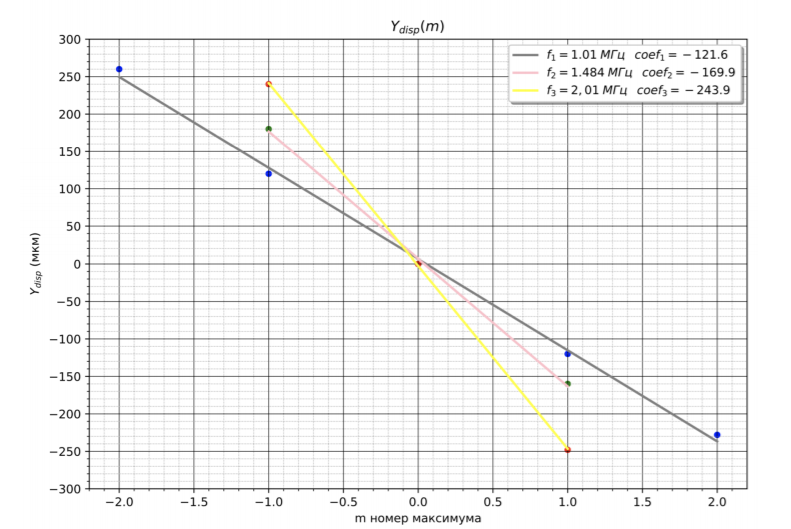
\includegraphics[scale = 0.8]{1.png}
	\end{center}
\end{figure}
\newpage
Поскольку $f = 28$ см, $\lambda = 6400 \pm 200$ ангстрем, то можно посчитать длину волны и скорость звука:

\begin{table}[h!]
	\begin{tabular}{|l|l|l|l|}
		\hline
		Частота, МГц     & 1.01     & 1.484    & 2.01     \\ \hline
		$\Lambda$, м      & 0.001473 & 0.001054 & 0.000734 \\ \hline
		$v$, м/с         & 1490     & 1570     & 1480     \\ \hline
		Погрешность, м/с & 47       & 49       & 56       \\ \hline
	\end{tabular}
\end{table}

\section{Определение скорости звука методом темного поля}

В результате измерений получаем таблицу результатов:

\begin{table}[h!]
	\begin{tabular}{|l|l|c|l|}
		\hline
		Частота, МГц & $N$ & \multicolumn{1}{l|}{$\Delta$} & $\Lambda$, м \\ \hline
		1.3          & 19  & 3.3         & 0.001234     \\ \cline{1-2} \cline{4-4} 
		1.6          & 23  &                              & 0.000938     \\ \cline{1-2} \cline{4-4} 
		1.8          & 27  &                              & 0.00075      \\ \cline{1-2} \cline{4-4} 
		2            & 29  &                              & 0.000697     \\ \cline{1-2} \cline{4-4} 
		2.2          & 32  &                              & 0.000783     \\ \hline
	\end{tabular}
\end{table}
\begin{figure}[h!]
	\begin{center}
		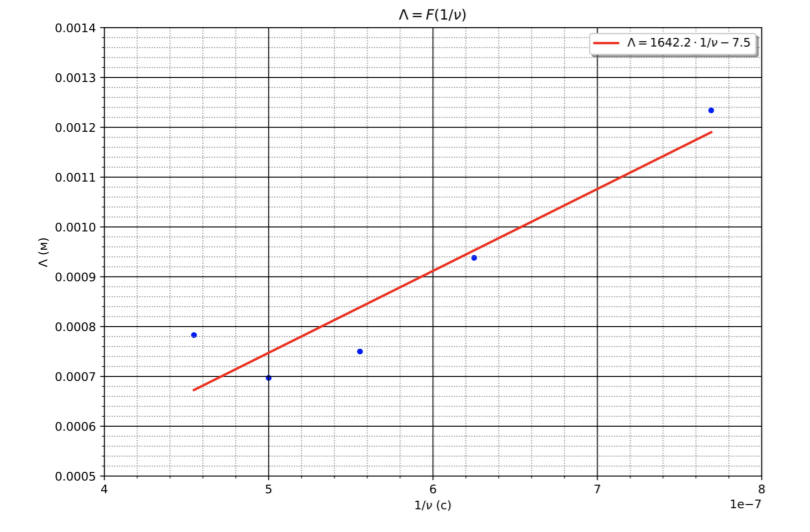
\includegraphics[scale = 0.67]{2.png}
	\end{center}
\end{figure}

В результате имеем $v = 1642 \pm 76$ м/c.
\end{document} % конец документа